% TEMPLATE for Usenix papers, specifically to meet requirements of
%  USENIX '05
% originally a template for producing IEEE-format articles using LaTeX.
%   written by Matthew Ward, CS Department, Worcester Polytechnic Institute.
% adapted by David Beazley for his excellent SWIG paper in Proceedings,
%   Tcl 96
% turned into a smartass generic template by De Clarke, with thanks to
%   both the above pioneers
% use at your own risk.  Complaints to /dev/null.
% make it two column with no page numbering, default is 10 point

% Munged by Fred Douglis <douglis@research.att.com> 10/97 to separate
% the .sty file from the LaTeX source template, so that people can
% more easily include the .sty file into an existing document.  Also
% changed to more closely follow the style guidelines as represented
% by the Word sample file. 

% Note that since 2010, USENIX does not require endnotes. If you want
% foot of page notes, don't include the endnotes package in the 
% usepackage command, below.

% This version uses the latex2e styles, not the very ancient 2.09 stuff.
\documentclass[letterpaper,twocolumn,10pt]{article}
\usepackage{usenix,hyperref,graphicx}
\begin{document}

%don't want date printed
\date{}

%make title bold and 14 pt font (Latex default is non-bold, 16 pt)
\title{\Large \bf Wonderful : A Terrific Application and Fascinating Paper}

\author{
{\rm Joshua Dawson}
\and
{\rm Peter Marheine}
\and
{\rm Frederico Rocha}
} % end author

\maketitle

% Use the following at camera-ready time to suppress page numbers.
% Comment it out when you first submit the paper for review.
%\thispagestyle{empty}

\subsection*{Abstract}

Blah blah blah.

\section{Introduction}

Blah blah blah.

\section{Related Work}

Blah blah blah.

Things like the SSL Observatory~\cite{ssl-observatory} and
VirusTotal's plugins~\cite{vtzilla,vtchromizer,vtexplorer}.

\section{Design}

Here's a typical figure reference.  The figure is centered at the
top of the column.  It's scaled.  It's explicitly placed.  You'll
have to tweak the numbers to get what you want.\\

% you can also use the wonderful epsfig package...
\begin{figure}[h]
    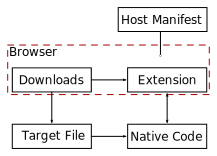
\includegraphics[width=\columnwidth]{system}
    \caption{This is a figure.}
    \label{fig:one}
\end{figure}

This text came after the figure, so we'll casually refer to \autoref{fig:one}
as we go on our merry way.

\section{Results}

Do we need this section?

\section{Discussion}

Blah blah blah.

\section{Limitations}

Blah blah blah.

\section{Conclusions}

Blah blah blah.

{\footnotesize \bibliographystyle{acm}
\bibliography{bibliography}}

\end{document}







